\section{Evaluation}
\label{sec:evaluation}

All the results presented in this section are obtained with the following parameters:
\begin{itemize}
    \item $n_D = 50$
    \item $n_{max} = 250$
    \item $N = 200$
\end{itemize}

\subsection{MinOver}
\begin{figure}[t]
	\centering
	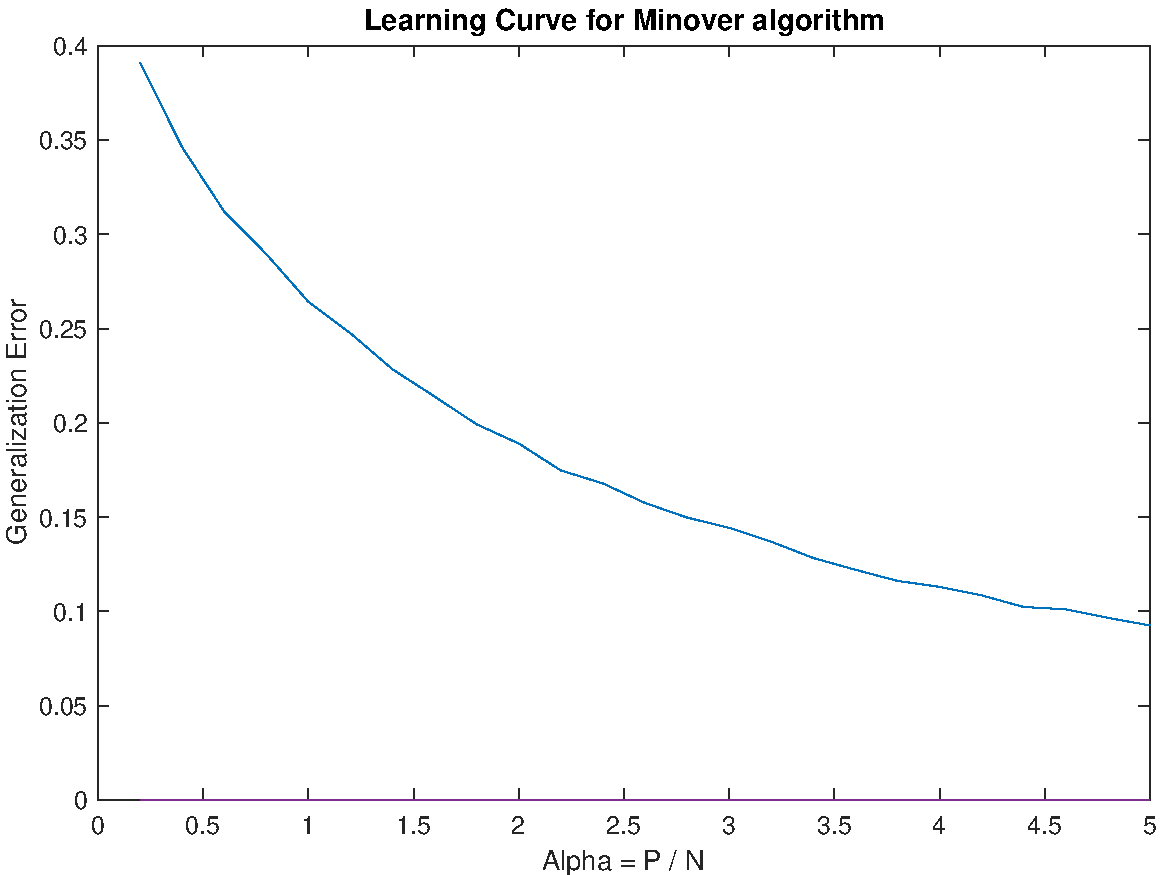
\includegraphics[width=\columnwidth]{figures/base}
    \caption{Generalization error of a perceptron trained with the MinOver algorithm on a linearly separable dataset.}
	\label{fig:base}
\end{figure}

\cref{fig:base} shows the generalization error of the perceptron trained with the MinOver algorithm on a linearly separable dataset (with no noise, $\lambda = 0$).
Since the number of dimensions of the dataset $N$ is fixed, $\alpha = P / N$ is proportional to the number of examples $P$ used for the training.
The generalization error decreases for higher values of $\alpha$, i.e. when the number of examples increases.
In other words, it seems to be the case:
$$\lim_{\alpha \to \infty} \bm{\mathsf{w}} = \bm{\mathsf{w}}^{*}$$

The examples are distributed in all the space and the boundary between the classes is fixed and determined by the teacher vector $\bm{\mathsf{w}}^{*}$.
Intuitively, for a higher number of examples $P$, the maximum margin between the $2$ classes decreases, since it is more likely that some example is really close to the boundary hyperplane determined by $\bm{\mathsf{w}}^{*}$.
Since the MinOver algorithm tries to find some separation hyperplane, it is easier to get closer to the teacher vector $\bm{\mathsf{w}}^{*}$ if the maximum possible margin is smaller.


\subsection{MinOver vs Rosenblatt}
\begin{figure}[t]
	\centering
	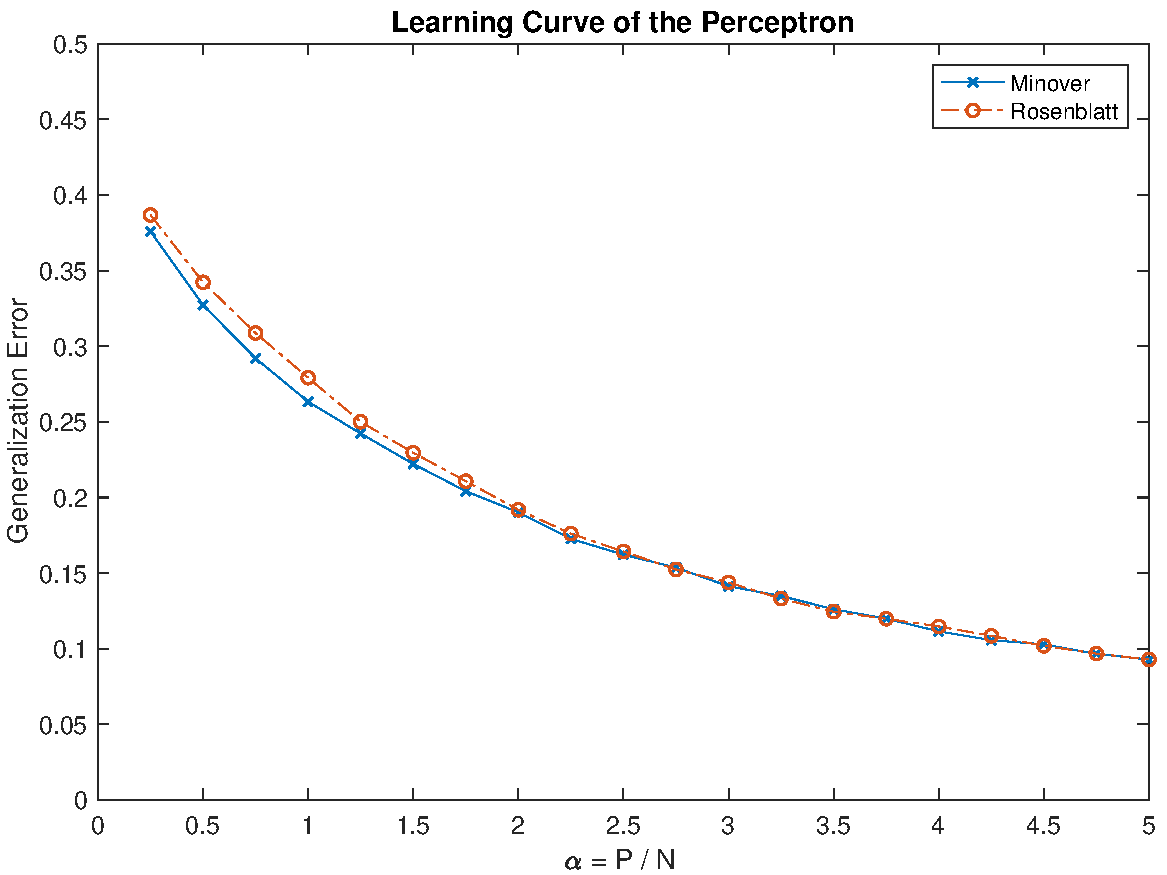
\includegraphics[width=\columnwidth]{figures/comparison}
    \caption{Generalization error for the MinOver and the Rosenblatt algorithms on a linearly separable dataset.}
	\label{fig:comparison}
\end{figure}

\cref{fig:comparison} shows the generalization error of the perceptron trained with the MinOver and the Rosenblatt algorithms on a linearly separable dataset (without noise, $\lambda = 0$).
For both algorithms the generalization error decreases with higher numbers of examples for the training (see the previous section).
In absence of noise, the performances of the $2$ algorithms are quite close, with MinOver performs slightly better than Rosenblatt for low values of $\alpha$.


\subsection{Noise}
\begin{figure}[t]
	\centering
	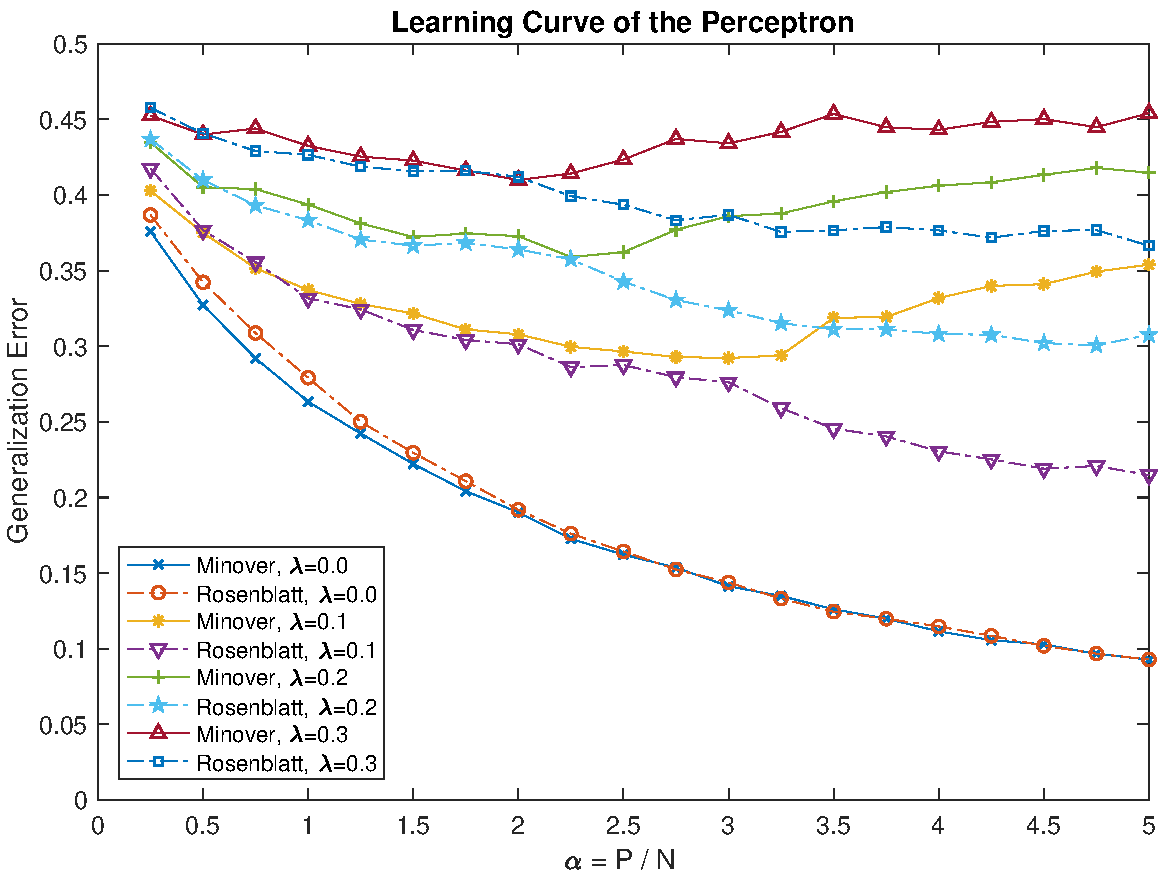
\includegraphics[width=\columnwidth]{figures/noise}
    \caption{Generalization error for the MinOver and the Rosenblatt algorithms on a noisy dataset. The dataset is generated starting from a linearly separable set of examples and swapping the labels of each example with probability $\lambda$. The lines for $\lambda = 0$ (no noise) are left as a reference.}
	\label{fig:noise}
\end{figure}

\cref{fig:noise} shows the generalization error of the perceptron trained with the MinOver and the Rosenblatt algorithms on a noisy dataset.
For both algorithms, the generalization error increases with the noise $\lambda$.

The error for the MinOver algorithm initially decreases by adding new examples, while it starts to increase again if the dataset gets bigger:
the algorithm diverges from the teacher vector $\bm{\mathsf{w}}^{*}$.
The more noise is present, the sooner the algorithm starts to diverge.
At each step, the algorithm selects the example with the lower stability $\kappa^\mu \propto \bm{\mathsf{w}} \cdotp \xi^\mu S^\mu_R$:
this quantity is positive for correctly classified examples and negative for wrongly classified ones.
If there are misclassified examples, the MinOver algorithm chooses one of them to update the weights vector $\bm{\mathsf{w}}$.
If the dataset is non linearly separable, the MinOver algorithm stacks forever:
each update can correct the classification for some point, but not for all of them;
in the following epochs, only the misclassified examples cause updates and create new wrongly classified point.
For the way it is constructed, the probability that the dataset is not linearly separable is non-zero (for $\lambda > 0$) and increases with $\alpha$.
For $\lambda = 0.3$, the algorithms has a generalization error of around $0.45$, very close to the error for a random guess.
The MinOver algorithm does not seem to be suitable for the classification of noisy data.

The Rosenblatt algorithm has similar performances, but it does not diverge when $\alpha$ increases.
In other words, the Rosenblatt algorithm is up to a certain degree able to generalize even for noisy training data.
